\section{Elliptical}

\subsection{Basic Equations}
% Area of A Sector of An Ellipse
% Deriving the Area of a Sector of an Ellipse
\begin{figure}[h]
\centering
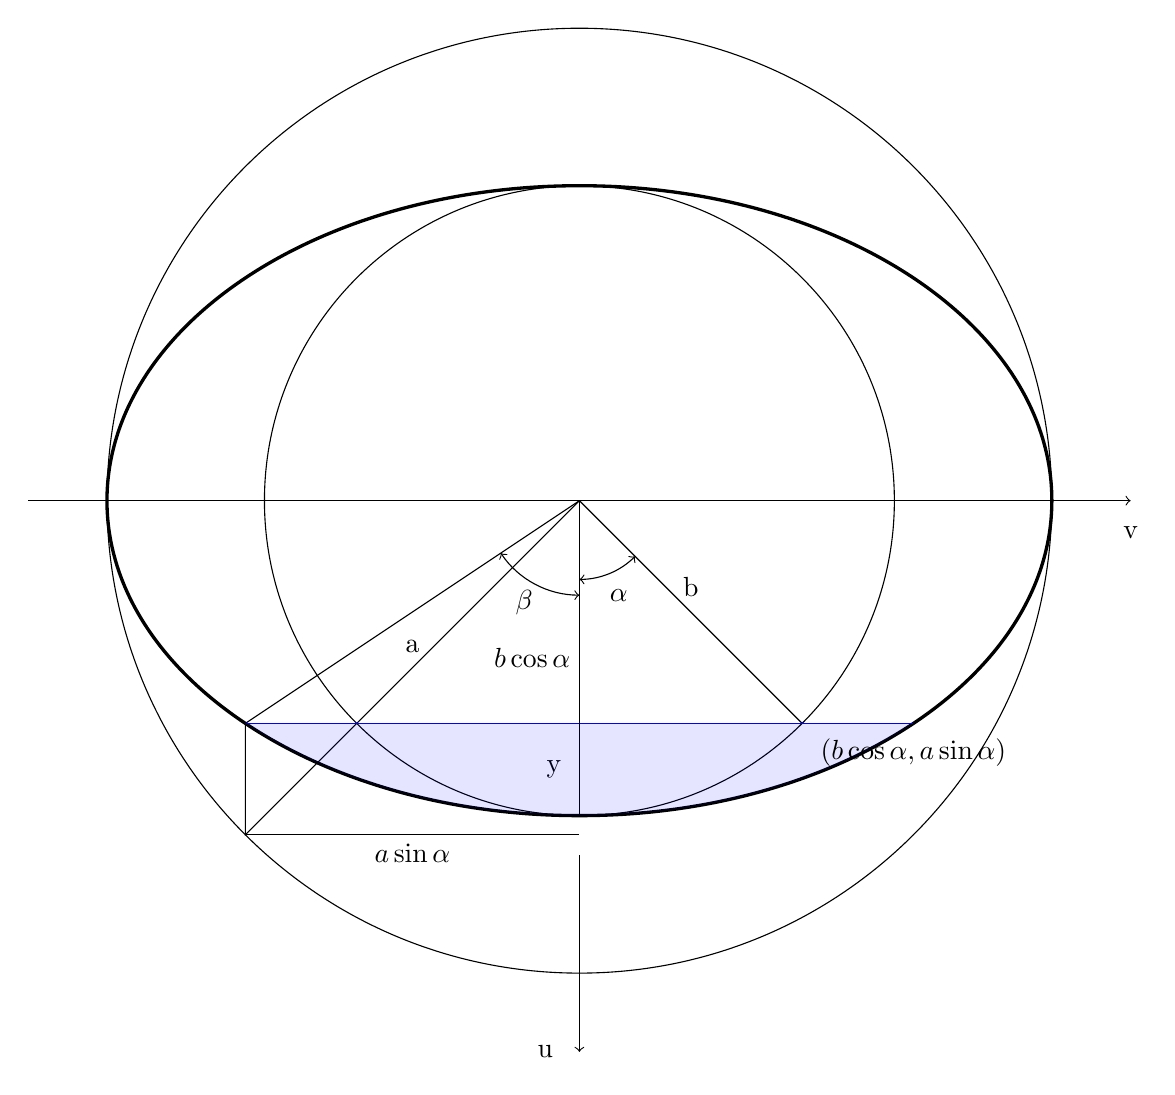
\begin{tikzpicture}

\draw (0,0) circle (6);
\draw (0,0) circle (4);
\draw [very thick](0,0) ellipse (6 and 4);

\draw[->](-7,0) --(7, 0) node[below =6]{v} ;
\draw[->](0, -4.5) --(0,-7) node[left =6]{u} ;


\draw (0,0)--node[above=2]{b} (2.828, -2.828);
\draw (0,0)--node[above=2]{a}(-4.242, -4.242)--(-4.242, -2.828);
\draw[blue] (-4.242, -2.828) -- (4.242, -2.828);
\draw (0,0)-- (0,-2.828)--node[left=3]{y} (0,-4);
\node at (-0.6, -2){$b\cos\alpha$};

\draw (-4.242, -4.242)--node[below]{$a\sin\alpha$}(0, -4.242);

\filldraw[fill=blue, opacity=0.1](-4.242, -2.828) arc[x radius=6, y radius = 4, start angle = 225, end angle=315];

\draw [<->] (0, -1) arc [radius=1, start angle=270, end angle=315];
\node at (0.5, -1.2) {$\alpha$};

\draw (0, 0) --(-4.242, -2.828);
\draw [<->] (0, -1.2) arc [radius=1.2, start angle=270, end angle=213.7];
\node at (-0.7, -1.3) {$\beta$};

\node at (4.242, -3.2) {$(b\cos\alpha, a\sin\alpha)$};

\end{tikzpicture}
\caption{Elliptical Section ($a \ge b$)}
\label{Fig:EllipseA}
\end{figure}

\begin{figure}[h]
\centering
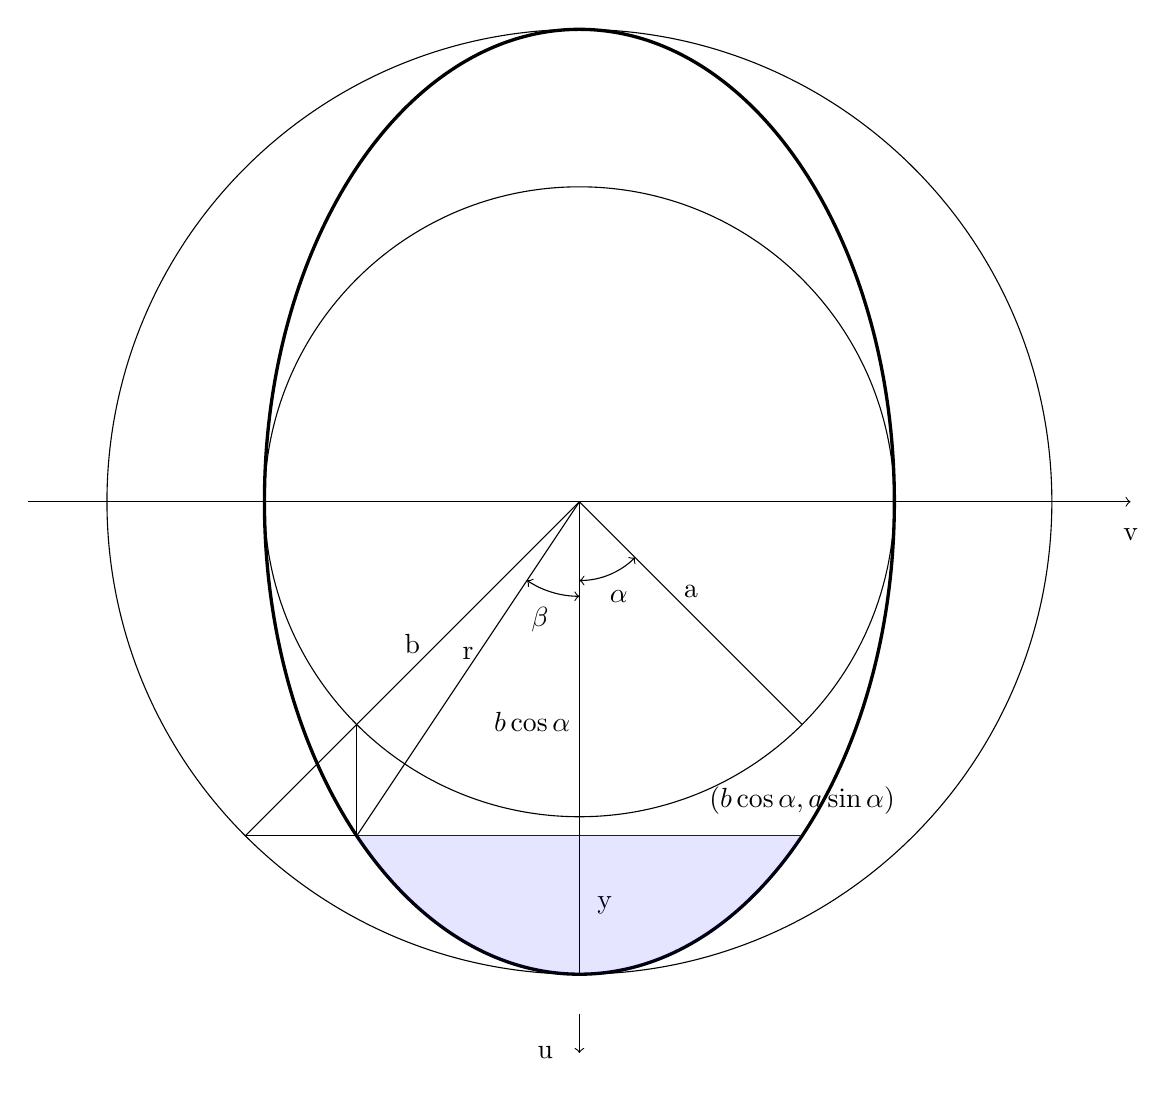
\begin{tikzpicture}
\draw (0,0) circle (6);
\draw (0,0) circle (4);
\draw [very thick](0,0) ellipse (4 and 6);
\draw[->](-7,0) --(7, 0) node[below =6]{v} ;
\draw[->](0, -6.5) --(0,-7) node[left =6]{u} ;

\draw (0,0)--node[above=2]{a} (2.828, -2.828);
\draw (0,0)--node[above=2]{b}(-4.242, -4.242);
\draw (-4.242, -4.242)--(-2.828, -4.242) -- (-2.828, -2.828);
\draw[blue] (-2.828, -4.242) --(2.828, -4.242);
\draw (0,-4.242)--node[right=3]{y} (0,-6);

\filldraw[fill=blue, opacity=0.1](-2.828, -4.242) arc[x radius=4, y radius = 6, start angle = 225, end angle=315];

\draw(0, 0) -- (0, -4.242);
\node at (-0.6, -2.8) {$b\cos\alpha$};

\draw [<->] (0, -1) arc [radius=1, start angle=270, end angle=315];
\node at (0.5, -1.2) {$\alpha$};

\draw [<->] (0, -1.2) arc [radius=1.2, start angle=270, end angle=236.31];
\node at (-0.5, -1.5) {$\beta$};


\draw (0, 0) --node[above]{r}(-2.828, -4.242);

\node at (2.828, -3.8) {$(b\cos\alpha, a\sin\alpha)$};

\end{tikzpicture}
\caption{Elliptical Section ($a < b$)}
\label{Fig:EllipseB}
\end{figure}

\begin{equation}
\begin{aligned}
u &= b\cos \alpha  \\
v &= a\sin \alpha  \\
\end{aligned}
\end{equation}

\begin{equation}
\tan\beta = \frac{a}{b}\tan\alpha
\end{equation}

\begin{equation}
\sin^2\alpha = \frac{\tan^2\alpha}{1+\tan^2\alpha}=\frac{b^2\tan^2\beta}{a^2+b^2\tan^2\beta} 
\end{equation}

\begin{equation}
\cos^2\alpha = \frac{1}{1+\tan^2\alpha}=\frac{a^2}{a^2+b^2\tan^2\beta}
\end{equation}

\begin{equation}
r^2 = a^2\sin^2\alpha + b^2\cos^2\alpha
\end{equation}

\begin{equation}
y = b(1 - \cos\alpha) 
\end{equation}

\begin{equation}
\cos\alpha =1 - \frac{y}{b}
\end{equation}

\begin{equation}
y' = \frac{\partial y}{\partial \alpha} = b \sin\alpha
\end{equation}

\subsection{Flow Area}
The flow area is
\begin{equation}
A = 2 \int_{b\cos\alpha }^b v du = -2ab\int^0_\alpha \sin^2tdt =  ab\int_0^\alpha (1 - \cos 2t) dt = ab(\alpha - \frac{1}{2}\sin 2 \alpha)
\end{equation}

\begin{equation}
A' = ab(1 - \cos2\alpha)
\end{equation}

\begin{equation}
A'' = 2ab\sin2\alpha
\end{equation}

\begin{equation}
\frac{\partial A}{\partial y} = \frac{A'}{y'} = 2a\sin\alpha = T_w
\end{equation}

\begin{equation}
\frac{\partial }{\partial \alpha}\left(\frac{\partial A}{\partial y}\right) = 2a\cos\alpha
\end{equation}

\begin{equation}
D_h = \frac{A'}{\frac{\partial A}{\partial y}} = \frac{b(\alpha - \frac{1}{2}\sin 2 \alpha)}{ 2\sin\alpha}
\end{equation}


\subsection{Wet Perimeter}
\subsubsection{$a \ge b$}
In the case of $a \ge b$ (Figure \ref{Fig:EllipseA}), the wet perimeter is
\begin{equation}
P =  2\int _0 ^{\alpha } \sqrt{a^2\cos^2t + b^2\sin^2t} dt =2 a\int _0 ^{\alpha } \sqrt{1 - \left(1 - b^2/a^2\right) \sin^2t} dt =  2aE(\alpha, \eta)
\end{equation}
with $\eta^2 = 1 - b^2/a^2$,  $E(\alpha, \zeta)$ as the Legendre ellitipcal integral of the second kind.

\begin{equation}
E(\alpha, \eta) = \alpha -\frac{1}{2}\eta^2\int_0^\alpha \sin^2 tdt - \frac{1}{2 \cdot 4}\eta^4\int_0^\alpha \sin^4 tdt - \frac{1 \cdot 3}{2 \cdot 4 \cdot 6}\eta^6\int_0^\alpha \sin^6 tdt + ...
\end{equation}

\begin{equation}
\begin{aligned}
\int \sin^n t dt &= -\frac{1}{n} \sin^{n-1} \cos t + \frac{n-1}{n} \int \sin^{n-2} t dt \\
\int_0^\alpha \sin^2 tdt &=  -\frac{1}{2}\sin \alpha \cos\alpha + \frac{1}{2}\alpha \\
\int_0^\alpha \sin^4 t dt &= -\frac{1}{4}\sin^3 \alpha  \cos \alpha + \frac{3}{4} \int_0^\alpha \sin^2 t dt \\
\int_0^\alpha \sin^6 t dt &= -\frac{1}{6}\sin^5 \alpha  \cos \alpha + \frac{5}{6} \int_0^\alpha \sin^4 t dt \\
\int_0^\alpha \sin^{2n} t dt &= -\frac{1}{2n}\sin^{2n-1} \alpha  \cos \alpha + \frac{2n-1}{2n} \int_0^\alpha \sin^{2n-2} t dt 
\end{aligned}
\end{equation}

\begin{center}
\begin{tabular}{| c | c | c | c | c | c | c | }
\hline
n & $a_n$ & $b_n$ & $c_n$ & $d_n$ & $e_n$ & $f_n$\\ 
\hline
1 & $-\frac{1}{2}\eta^2$              &  $-\frac{1}{2}$    & $\sin\alpha \cos\alpha$ &  $\frac{1}{2}$        & $b_1c_1 + d_1\alpha$   & $a_1e_1$ \\ 
2 & $a_1 \frac{\eta^2}{4}$          &  $-\frac{1}{4}$    &  $c_1 \sin^2\alpha$       &  $\frac{3}{4}$        & $b_2c_2 + d_2e_1$       & $a_2e_2$   \\  
3 & $a_2 \frac{\eta^2}{6}$          &  $-\frac{1}{6}$    &  $c_2 \sin^2\alpha$       &  $\frac{5}{6}$        & $b_3c_3 + d_3e_2$       & $a_3e_3$   \\  
n & $a_{n-1} \frac{\eta^2}{2n}$ &   $-\frac{1}{2n}$ &  $c_{n-1} \sin^2\alpha$ & $\frac{2n-1}{2n}$ & $b_nc_n + d_ne_{n-1}$ & $a_ne_n$  \\
\hline
\end{tabular}
\end{center}



\subsubsection{$a < b$}

For $a < b$, the wet perimeter is (Figure \ref{Fig:EllipseB})
\begin{equation}
P =  2\int _0 ^{\alpha } \sqrt{a^2\cos^2t + b^2\sin^2t} dt = 2b\int _0 ^{\alpha } \sqrt{1 - \left(1 - a^2/b^2\right) \cos^2t} dt =  2bF(\alpha, \zeta)
\end{equation}
with $\zeta^2 = 1 - a^2/b^2$.

\begin{equation}
F(\alpha, \eta) = \alpha - \frac{1}{2}\zeta^2\int_0^{\alpha} \cos ^2 t dt - \frac{1}{2^2 \cdot 2!}\zeta^4\int_0^{\alpha} \cos ^4 t dt - \frac{1 \cdot 3}{2^3 \cdot 3!}\zeta^6\int_0^{\alpha} \cos ^6 t dt - \cdot \cdot \cdot
\end{equation}

\begin{equation}
\begin{aligned}
\int \cos^n t dt &= \frac{1}{n} \sin t  \cos^{n-1} t + \frac{n}{n-1} \int \cos^{n-2} t dt \\
\int_0^\alpha \cos^2 t dt &= \frac{1}{2}\sin \alpha  \cos \alpha + \frac{1}{2} \alpha  \\
\int_0^\alpha \cos^4 t dt &= \frac{1}{4}\sin \alpha  \cos^3 \alpha + \frac{3}{4} \int_0^\alpha \cos^2 t dt \\
\int_0^\alpha \cos^6 t dt &= \frac{1}{6}\sin \alpha  \cos^5 \alpha + \frac{5}{6} \int_0^\alpha \cos^4 t dt \\
\int_0^\alpha \cos^{2n} t dt &= \frac{1}{2n}\sin \alpha  \cos^{2n-1} \alpha + \frac{2n-1}{2n} \int_0^\alpha \cos^{2n-2} t dt 
\end{aligned}
\end{equation}

For both cases,

\begin{equation}
P' = 2\sqrt{a^2\cos^2\alpha + b^2\sin^2\alpha} 
\end{equation}

\begin{equation}
P'' =-\frac{(a^2-b^2)\sin2\alpha}{\sqrt{a^2\sin^2\alpha + b^2\cos^2\alpha}} 
\end{equation}

\noindent Neton's method is used to calculate normal depth $y_n$,  critical depth $y_c$, $\alpha_{max}$, $y_{max}$, and $Q_{max}$.
%\begin{equation}
%\cos \alpha =1 - y/b 
%\end{equation}

%\begin{figure}[h]
%\centering
%\begin{tikzpicture}

%\draw (0,0) circle (3);
%\draw (0,0) circle (2);
%\draw [very thick](0,0) ellipse (3 and 2);


%\draw (0,0)--node[above=2]{b} (1.41421, -1.41421);
%\draw (0,0)--node[above=2]{a}(-2.12132, -2.12132)--(-2.12132, -1.41421);
%\draw[blue] (-2.12132, -1.41421) -- (2.12132, -1.41421);
%\draw (0,-1.41421)--node[right=3]{y} (0,-2);

%\filldraw[fill=blue, opacity=0.2](-2.12132, -1.41421) arc[x radius=3, y radius = 2, start angle = 225, end angle=315];

%\draw [<->] (-0.3536, -0.3536) arc [radius=0.5, start angle=225, end angle=315];
%\node at (-0.0, -0.8) {$\theta=2\alpha$};

%\node at (0.0, -3.5) {$(a) a > b$};

%\draw (7,0) circle (3);
%\draw (7,0) circle (2);
%\draw [very thick](7,0) ellipse (2 and 3);

%\draw (7,0)--node[above=2]{a} (8.41421, -1.41421);
%\draw (7,0)--node[above=2]{b}(4.87868, -2.12132)--(5.58579, -2.12132)--(5.58579,-1.41421);
%\draw[blue] (5.58579, -2.12132) --(8.41421, -2.12132);
%\draw (7,-2.12132)--node[right=3]{y} (7,-3);

%\filldraw[fill=blue, opacity=0.2](5.58579, -2.12132) arc[x radius=2, y radius = 3, start angle = 225, end angle=315];

%\draw [<->] (6.6465, -0.3536) arc [radius=0.5, start angle=225, end angle=315];
%\node at (7, -0.8) {$\theta=2\alpha$};

%\node at (7.0, -3.5) {$(b) a < b$};

%\end{tikzpicture}
%\end{figure}

%\subsection{Calculate Maximum Discharge Using Manning's Equation}
%\begin{equation}  
%Q = \frac{K_u}{n}AR^{2/3}S^{1/2} = \frac{K_u}{n}A^{5/3}P^{-2/3}S^{1/2},
%\end{equation}

%\begin{equation}  
%\frac{dQ}{d\theta} = \frac{K_u}{n} \left(\frac{5}{3}R^{2/3}\frac{\partial A}{\partial \theta} -  \frac{2}{3}R^{5/3}\frac{\partial P}{\partial \theta} \right) S^{1/2}=0,
%\end{equation}
%To reach maximum capacity, the $\alpha$ is solved using Newton-Raphson method

%\begin{equation}  
%\alpha _{i+1} = \alpha _i - \frac{f(\alpha _i)}{f'(\alpha_i)},
%\end{equation}

%with Eq. \ref{Eq:CircularMaxQ},

%\begin{equation}  
%f(\alpha) = 5A'P -  2AP' = 0,
%\end{equation}
%and
%\begin{equation}  
%f'(\alpha) = 3A'P' + 5A''P - 2AP''.
%\end{equation}

%\subsection{Calculate Normal Depth}
%For $Q$ less than $Q_{max}$,
%\begin{equation}  
%\alpha_{i+1} = \alpha_i -\frac{f_d(\alpha_{i})}{f'_d(\alpha_{i})}
%\end{equation}
%where
%\begin{equation}  
%f_d(\alpha_{i})= \frac{K_u}{n}A^{5/3}P^{-2/3}S^{1/2} - Q 
%\end{equation}

%\begin{equation}  
%f'_d(\alpha_{i})= \frac{K_u}{n}\left(\frac{5}{3}R^{2/3}A' -  \frac{2}{3}R^{5/3}P'\right)S^{1/2}
%\end{equation}



%\subsection{Calculate Critical Depth}

%\begin{equation}  
%\frac{\partial A}{\partial y} (\alpha)= \frac{\frac{\partial A}{\partial \alpha}}{\frac{\partial y}{\partial \alpha}}=\frac{ab(1 - \cos2\alpha)}{b\sin \alpha} = 2a\sin \alpha
%\end{equation}

%\begin{equation}  
%\frac{\partial}{\partial \alpha} \left(\frac{\partial A}{\partial y} \right) =2  a \cos \alpha
%\end{equation}


%\begin{equation}  
%f_c(\alpha)= gA^3 - Q^2\frac{\partial A}{\partial y} =  gA^3 - 2aQ^2 \sin\alpha
%\end{equation}

%\begin{equation}  
%f'_c(\alpha)= 3gA^2\frac{\partial A}{\partial \alpha} - Q^2\frac{\partial}{\partial \alpha} \left(\frac{\partial A}{\partial y} \right)
%\end{equation}

